\documentclass[aspectratio=169]{beamer}

% The talk on the note (report/gatqsat.tex), in English; gatqsat-talk-it.tex
% defines \italian and inputs this file, so that the Italian deck is the same
% file with the other text of each \T{english}{italiano} pair.
\ifdefined\italian
  \usepackage[italian]{babel}
  \newcommand{\T}[2]{#2}
\else
  \usepackage[english]{babel}
  \newcommand{\T}[2]{#1}
\fi

% the lamalunga theme, with the violet of the decks of the project as the
% primary; every other color, size and spacing follows from it
\usetheme[aspect=beamer, primary=665094, sectionpage=none, spiral=false]{lamalunga}
\usepackage{amsmath,amssymb}
\usepackage{booktabs}
% the links to the papers and to the code in the primary, so that one sees
% they can be clicked; the internal links keep the color of the text
\hypersetup{colorlinks=true, linkcolor=., urlcolor=lamalunga-primary}
% the backgrounds (img/make_backgrounds.py of GQSAT), faded: a wall of clauses
% with the AND and the OR of the CNF behind the title page, and neighborhoods
% whose messages are weighted by attention behind every other frame
\setbeamertemplate{background}{%
  \begin{tikzpicture}
    \useasboundingbox (0,0) rectangle (\paperwidth,\paperheight);
    \ifnum\value{page}>1
      \node[anchor=center, inner sep=0pt, opacity=0.3] at (0.5\paperwidth,0.5\paperheight)
        {\includegraphics[width=\paperwidth, height=\paperheight]{bg-content.pdf}};
    \else
      \node[anchor=center, inner sep=0pt, opacity=0.4] at (0.5\paperwidth,0.5\paperheight)
        {\includegraphics[width=\paperwidth, height=\paperheight]{bg-cover.pdf}};
    \fi
  \end{tikzpicture}}
% the figures are those of the note
\graphicspath{{img/}{../report/img/}}

% \upd{...} marks a number that the Colab campaign will change, as in the note
\newcommand{\upd}[1]{#1}

% a section divider: a box of the primary in the minor part of the golden
% section of the page (38.2% at the right), inside the margins, with the
% title centred in it; the content of the section, centred, in the major part
\newlength\dividerbox \setlength\dividerbox{\goldenminor{\paperwidth}}
\addtolength\dividerbox{-\lamalungahmargin}
\newlength\dividerboxheight \setlength\dividerboxheight{\paperheight}
\addtolength\dividerboxheight{-2\lamalungavmargin}
\newlength\dividerleft \setlength\dividerleft{\goldenmajor{\paperwidth}}
\addtolength\dividerleft{-2\lamalungahmargin}
\newcommand{\sectiondivider}[3]{%
\begin{frame}[plain]
  \begin{tikzpicture}[remember picture, overlay]
    \node[anchor=north east, inner sep=0pt, minimum width=\dividerbox,
      minimum height=\dividerboxheight, fill=lamalunga-primary,
      text=lamalunga-on-primary, align=center,
      text width=\dimexpr\dividerbox-2\fib{6}pt\relax,
      font=\lamalungatitlefamily\fontseries{eb}\selectfont\modularsize{0.5}]
      at ([xshift=-\lamalungahmargin, yshift=-\lamalungavmargin]current page.north east)
      {\lamalunganohyphens #1};
  \end{tikzpicture}%
  \begin{minipage}[c][\dividerboxheight][c]{\dividerleft}
    \vspace*{\fill}
    #2
    \vspace*{\fill}
    {\modularsize{-1}\color{lamalunga-muted}#3\par}
  \end{minipage}
\end{frame}}

% a long title: one step below the default, so that it fits the first
% square of the spiral
\setbeamerfont{title}{size=\modularsize{1}}

% the title without \T, so that the title page sees the \\
\ifdefined\italian
  \title{Attenzione su grafo in un'euristica\\ di branching appresa per SAT}
\else
  \title{Graph Attention in a Learned\\ Branching Heuristic for SAT}
\fi
\subtitle{\T{GAT-Q-SAT against Graph-Q-SAT, at matched training set and with two controls}%
            {GAT-Q-SAT contro Graph-Q-SAT, a parit\`a di training set e con due controlli}}
\author{\textcolor{lamalunga-primary}{Donato Meoli}}
\institute{\textcolor{lamalunga-accent}{Universit\`a di Pisa}}
\date{}

\begin{document}

\maketitle

% ==================================================================== problem
\begin{frame}{\T{The branching heuristic of a CDCL solver}{L'euristica di branching di un solutore CDCL}}
  \begin{itemize}
    \item \T{A CDCL solver repeatedly decides the value of a variable, propagates, and on a
          conflict learns a clause and backjumps; the choice of the decision is left to a
          heuristic, usually VSIDS, which ranks the variables by activity counters.}%
          {Un solutore CDCL decide ripetutamente il valore di una variabile, propaga, e a ogni
          conflitto impara una clausola e fa backjump; la scelta della decisione \`e lasciata a
          un'euristica, di solito VSIDS, che ordina le variabili con contatori di attivit\`a.}
    \item \T{The counters carry little information at the start of the search, and a poor
          decision costs time but never correctness: the heuristic is a natural place for a
          learned policy.}%
          {All'inizio della ricerca i contatori dicono poco, e una decisione sbagliata costa
          tempo ma non correttezza: l'euristica \`e il posto naturale per una politica appresa.}
    \item \T{Graph-Q-SAT (Kurin et al., 2020) learns it by Deep Q-Learning on the bipartite
          graph of the formula, and sums the messages of all the neighbors of a node with the
          same weight.}%
          {Graph-Q-SAT (Kurin et al., 2020) la impara con il Deep Q-Learning sul grafo
          bipartito della formula, e somma i messaggi di tutti i vicini di un nodo con lo
          stesso peso.}
    \item \T{This work adds graph attention to its core block (GAT-Q-SAT), and asks where
          weighting the neighbors helps, and whether the gain comes from the attention or
          from the added parameters.}%
          {Questo lavoro aggiunge l'attenzione su grafo al suo blocco centrale (GAT-Q-SAT), e
          si chiede dove pesare i vicini aiuti, e se il guadagno venga dall'attenzione o dai
          parametri in pi\`u.}
  \end{itemize}
\end{frame}

% ==================================================================== MDP
\sectiondivider{\T{The method}{Il metodo}}{%
  \begin{itemize}
    \item \T{Branching as a decision process}{Il branching come processo decisionale}
    \item Graph-Q-SAT
    \item GAT-Q-SAT
    \item \T{The two controls}{I due controlli}
  \end{itemize}}{%
  \href{https://arxiv.org/abs/1909.11830}{Kurin et al., \emph{Can Q-Learning with Graph
  Networks Learn a Generalizable Branching Heuristic for a SAT Solver?}}\\
  \href{https://arxiv.org/abs/1710.10903}{Veli\v{c}kovi\'c et al., \emph{Graph Attention Networks}}.}

\begin{frame}{\T{Branching as a decision process}{Il branching come processo decisionale}}
  \begin{itemize}
    \item \T{The state is the formula simplified by the partial assignment, with the learned
          clauses; an action is an unassigned variable with a truth value; a step is one
          decision with the propagation and the conflict analysis it triggers.}%
          {Lo stato \`e la formula semplificata dall'assegnamento parziale, con le clausole
          imparate; un'azione \`e una variabile libera con un valore di verit\`a; un passo \`e
          una decisione con la propagazione e l'analisi dei conflitti che ne seguono.}
    \item \T{The reward is $-0.1$ at each step and $0$ at termination, so that maximizing the
          return means terminating in as few decisions as possible.}%
          {La ricompensa \`e $-0.1$ a ogni passo e $0$ alla fine, quindi massimizzare il
          ritorno vuol dire terminare con il minor numero di decisioni.}
    \item \T{DQN approximates}{DQN approssima}
          $Q^\star(s,a) = \mathbb E\big[r + \gamma \max_{a'} Q^\star(s',a')\big]$
          \T{with a target network and a uniform replay buffer, and the heuristic is}%
          {con una target network e un replay buffer uniforme, e l'euristica \`e}
          $\pi(s) = \arg\max_a Q_\theta(s,a)$.
    \item \T{The number of actions changes along an episode and the state is defined up to
          a permutation of variables and clauses: hence a graph network, which scores each
          variable node and applies to formulas of any size.}%
          {Il numero di azioni cambia lungo un episodio e lo stato \`e definito a meno di
          permutazioni di variabili e clausole: di qui una rete su grafo, che d\`a un punteggio
          a ogni nodo variabile e si applica a formule di qualunque dimensione.}
  \end{itemize}
  {\footnotesize\color{lamalunga-muted}\T{Configuration of Kurin et al.: Adam at $2\cdot10^{-5}$,
  $\gamma=0.99$, buffer of 20000, minibatches of 64, 50000 updates, at most 500 decisions of
  the model per episode (the cap).}{Configurazione di Kurin et al.: Adam a $2\cdot10^{-5}$,
  $\gamma=0.99$, buffer di 20000, minibatch di 64, 50000 aggiornamenti, al pi\`u 500 decisioni
  del modello per episodio (il cap).}\par}
\end{frame}

% ==================================================================== Graph-Q-SAT
\begin{frame}{Graph-Q-SAT}
  \begin{columns}[c]
    \begin{column}{0.42\textwidth}
      \footnotesize
      \T{Nodes: the free variables and the clauses not yet satisfied; edges: the occurrences,
      with the polarity.}{Nodi: le variabili libere e le clausole non ancora soddisfatte;
      archi: le occorrenze, con la polarit\`a.}
      \T{A core block, applied $M=4$ times with shared weights, updates the edges, the nodes
      and the global attribute:}{Un blocco centrale, applicato $M=4$ volte con pesi condivisi,
      aggiorna gli archi, i nodi e l'attributo globale:}
      \begin{align*}
        e_{ij}' &= \phi^e(e_{ij}, v_i, v_j, u)\\
        v_i'    &= \phi^v\big(\textstyle\sum_{j\in\mathcal N_i} e_{ij}', v_i, u\big)\\
        u'      &= \phi^u(\bar e', \bar v', u)
      \end{align*}
      \T{The sum gives the same weight to all the clauses of a variable; 71144 parameters.}%
      {La somma d\`a lo stesso peso a tutte le clausole di una variabile; 71144 parametri.}
    \end{column}
    \begin{column}{0.58\textwidth}
      \centering
      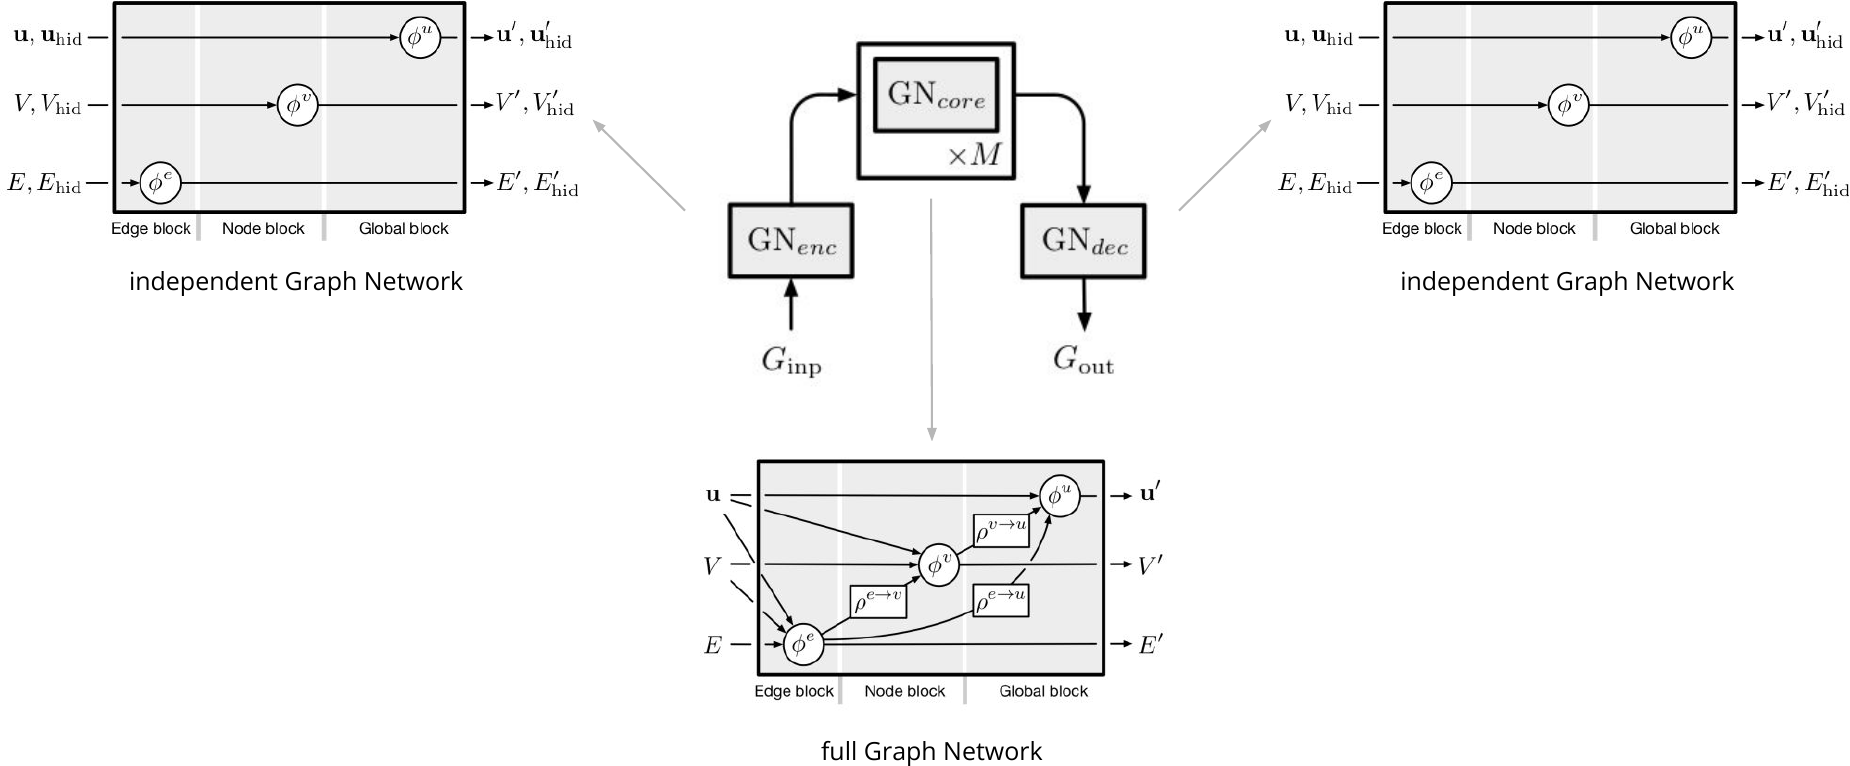
\includegraphics[width=\textwidth]{gqsat_epd.png}\\
      {\scriptsize \T{encoder, core block $\times M$, decoder (after Battaglia et al.)}%
      {encoder, blocco centrale $\times M$, decoder (da Battaglia et al.)}}
    \end{column}
  \end{columns}
\end{frame}

% ==================================================================== GAT-Q-SAT
\begin{frame}{GAT-Q-SAT}
  \begin{columns}[c]
    \begin{column}{0.42\textwidth}
      \footnotesize
      \T{Two edge-featured attention layers between the node and the global update
      (3 heads, then 1):}{Due strati di attenzione con le feature degli archi fra
      l'aggiornamento dei nodi e quello globale (3 teste, poi 1):}\par\scriptsize
      \begin{align*}
        v_i^{+} &= \textstyle\big\|_{k} \sum_{j \in \mathcal N_i} \alpha^k_{ij}\, W_k v_j + b\\
        \alpha^k_{ij} &\propto \exp \mathrm{LeakyReLU}\big(\mathbf w_k^{\!\top}
            [W_k v_i \,\|\, W_k v_j \,\|\, W^e_k e'_{ji}]\big)
      \end{align*}
      \footnotesize
      \T{The coefficients depend on the current edge embeddings, which carry the polarity
      and what the block has added to it. 113256 parameters, about 60\% more.}%
      {I coefficienti dipendono dagli embedding correnti degli archi, che portano la
      polarit\`a e ci\`o che il blocco vi ha aggiunto. 113256 parametri, circa il 60\% in pi\`u.}
    \end{column}
    \begin{column}{0.58\textwidth}
      \centering
      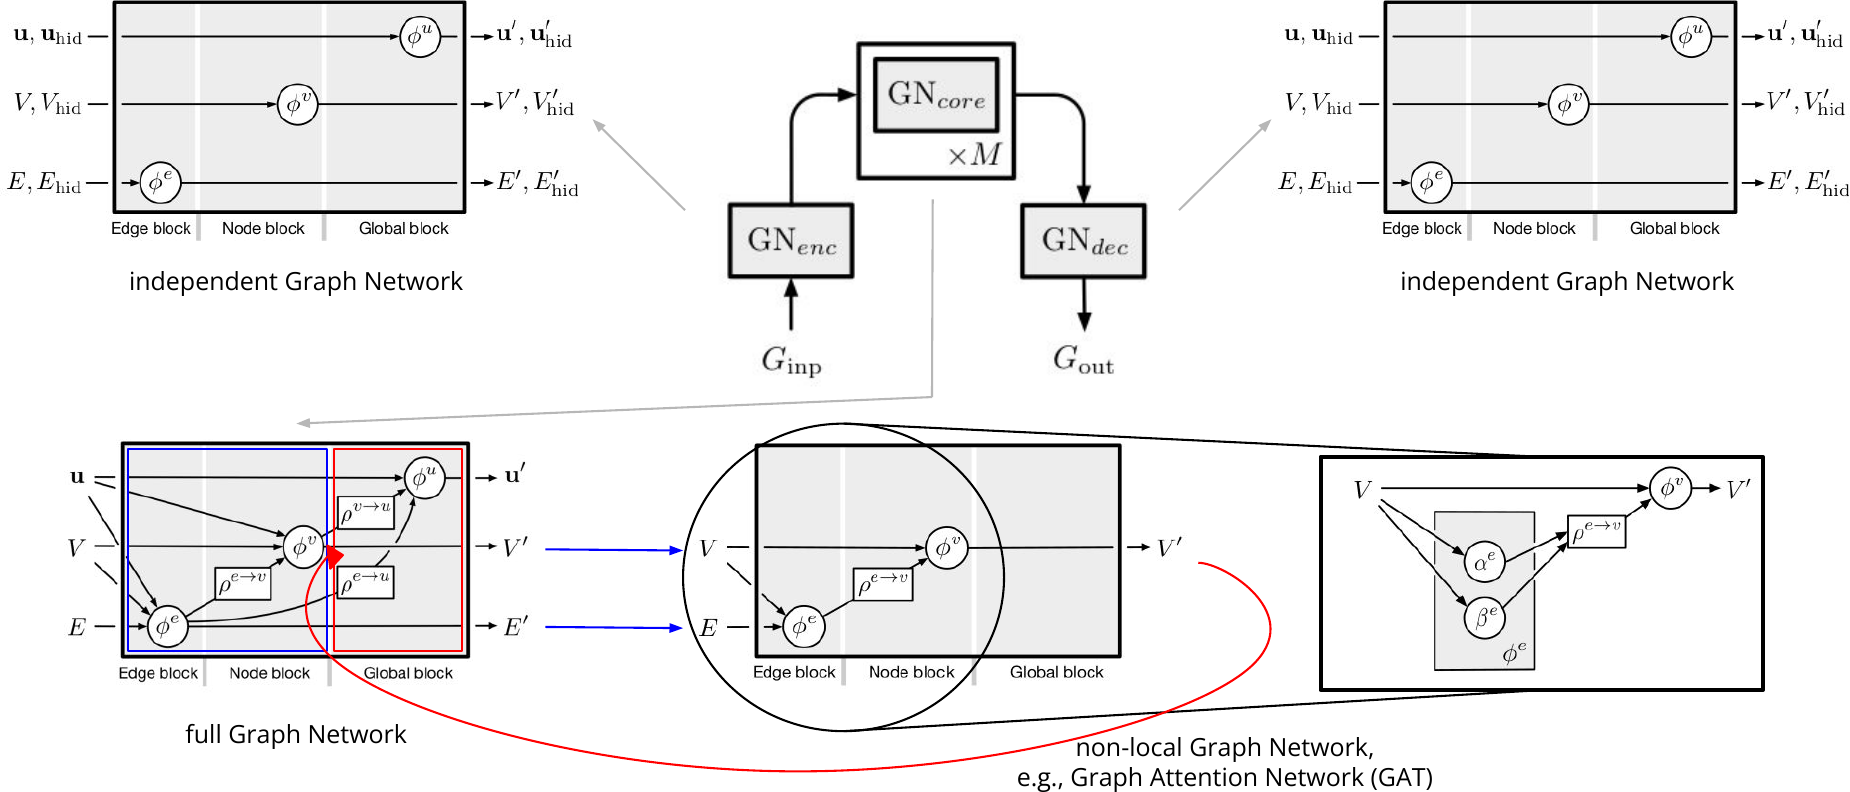
\includegraphics[width=\textwidth]{gatqsat_epd.png}\\
      {\scriptsize \T{the core block with a non-local block inserted}%
      {il blocco centrale con un blocco non locale inserito}}
    \end{column}
  \end{columns}
\end{frame}

% ==================================================================== controls
\begin{frame}{\T{Attention or capacity: the two controls}{Attenzione o capacit\`a: i due controlli}}
  \T{GAT-Q-SAT adds the attention to the sum, so a gain may be due to the attention or
  simply to the larger network. Two more models, with the same configuration:}%
  {GAT-Q-SAT aggiunge l'attenzione alla somma, quindi un guadagno pu\`o venire
  dall'attenzione o semplicemente dalla rete pi\`u grande. Altri due modelli, con la stessa
  configurazione:}
  \begin{itemize}
    \item \T{Graph-Q-SAT wide: hidden layers of 104 units in place of 64, the capacity of
          GAT-Q-SAT with no attention;}%
          {Graph-Q-SAT wide: strati nascosti di 104 unit\`a invece di 64, la capacit\`a di
          GAT-Q-SAT senza attenzione;}
    \item \T{attention aggregation: the sum replaced by a mean weighted by attention (3 heads,
          averaged), at the capacity of Graph-Q-SAT.}%
          {attention aggregation: la somma sostituita da una media pesata dall'attenzione (3
          teste, mediate), alla capacit\`a di Graph-Q-SAT.}
  \end{itemize}
  \begin{center}\footnotesize\setlength{\tabcolsep}{4pt}
  \begin{tabular}{lcccc}
    \toprule
     & Graph-Q-SAT & Graph-Q-SAT wide & attention aggregation & GAT-Q-SAT \\
    \midrule
    \T{parameters}{parametri} & 71144 & 113504 & 71627 & 113256 \\
    \T{training seeds}{semi di training} & 3 & 2 & 2 & 3 \\
    \bottomrule
  \end{tabular}
  \end{center}
\end{frame}

% ==================================================================== port
\sectiondivider{\T{Port and setup}{Port e impostazione}}{%
  \begin{itemize}
    \item \T{The port to the current stack}{Il port allo stack attuale}
    \item \T{The measure and the reference solver}{La misura e il solutore di riferimento}
  \end{itemize}}{}

\begin{frame}{\T{The port, and a test of what it computes}{Il port, e una prova di ci\`o che calcola}}
  \begin{itemize}
    \item \T{The code of 2020 is written for PyTorch~1.1 with pinned compiled extensions
          (\texttt{torch-scatter}, \texttt{torch-sparse}), which can no longer be installed:
          I ported it to the current PyTorch and PyTorch Geometric.}%
          {Il codice del 2020 \`e scritto per PyTorch~1.1 con estensioni compilate a versione
          fissa (\texttt{torch-scatter}, \texttt{torch-sparse}), che non si installano pi\`u:
          l'ho portato alle versioni attuali di PyTorch e PyTorch Geometric.}
    \item \T{The aggregations come from \texttt{torch\_geometric.utils.scatter}; the
          environment runs with \texttt{gym} and \texttt{gymnasium}; the MiniSat wrapper is
          rebuilt against \texttt{numpy}~2; the checkpoints of 2021 load with the current
          \texttt{GATConv}.}%
          {Le aggregazioni vengono da \texttt{torch\_geometric.utils.scatter}; l'ambiente gira
          con \texttt{gym} e con \texttt{gymnasium}; il wrapper di MiniSat \`e ricompilato
          su \texttt{numpy}~2; i checkpoint del 2021 si caricano con il \texttt{GATConv}
          attuale.}
    \item \T{The checkpoints of 2021, evaluated on the new stack, give the same iterations
          as in 2021 on every instance in 63 of 86 evaluations, and medians within $0.03$ in
          the others (on \texttt{flat30-60}: $1.833$ and $2.000$ on both stacks).}%
          {I checkpoint del 2021, valutati sul nuovo stack, danno le stesse iterazioni del
          2021 su ogni istanza in 63 valutazioni su 86, e mediane entro $0.03$ nelle altre (su
          \texttt{flat30-60}: $1.833$ e $2.000$ su entrambi gli stack).}
    \item \T{The training path was checked by retraining the two coloring models from scratch
          (the seeds of 2026).}%
          {Il training \`e stato verificato riaddestrando da zero i due modelli sul coloring (i
          semi del 2026).}
  \end{itemize}
\end{frame}

\begin{frame}{\T{The measure and the reference solver}{La misura e il solutore di riferimento}}
  \begin{columns}[t]
    \begin{column}{0.5\textwidth}
      \[
        \mathrm{MRIR}=\operatorname{median}
        \frac{\#\text{\T{iterations of MiniSat}{iterazioni di MiniSat}}}
             {\#\text{\T{iterations of the model}{iterazioni del modello}}}
      \]
      \T{over the instances of a family; an iteration is a decision, of the model or of
      VSIDS, which takes over after the cap ($500$ unless stated otherwise). Above $1$ the
      model takes fewer decisions than MiniSat.}%
      {sulle istanze di una famiglia; un'iterazione \`e una decisione, del modello o di
      VSIDS, che subentra dopo il cap ($500$ se non detto altrimenti). Sopra $1$ il modello
      prende meno decisioni di MiniSat.}
    \end{column}
    \begin{column}{0.5\textwidth}
      \begin{itemize}
        \item \T{The model drives MiniSat without restarts; the denominator is the stronger
              MiniSat on each family: with restarts on coloring (up to 26\% fewer
              iterations), without on uniform random 3-SAT (2.2 to 2.9 times fewer at 250
              variables).}%
              {Il modello guida MiniSat senza restart; al denominatore c'\`e il MiniSat pi\`u
              forte su ogni famiglia: con i restart sul coloring (fino al 26\% di iterazioni in
              meno), senza sul random 3-SAT uniforme (da 2.2 a 2.9 volte meno a 250 variabili).}
        \item \T{100 test instances per family; graph coloring from 30 to 200 nodes, trained
              on 50.}%
              {100 istanze di test per famiglia; coloring da 30 a 200 nodi, addestrato su 50.}
      \end{itemize}
    \end{column}
  \end{columns}
\end{frame}

% ==================================================================== results
\sectiondivider{\T{Results}{Risultati}}{%
  \begin{itemize}
    \item \T{Graph coloring, by size}{Graph coloring, per dimensione}
    \item \T{Capacity or attention}{Capacit\`a o attenzione}
    \item \T{A change of the training distribution}{Un cambio della distribuzione di training}
    \item \T{A change of domain}{Un cambio di dominio}
    \item \T{Uniform random 3-SAT}{Random 3-SAT uniforme}
    \item \T{Iterations and running time}{Iterazioni e tempo}
  \end{itemize}}{}

\begin{frame}{\T{Graph coloring: the gap grows with the size}{Graph coloring: il divario cresce con la dimensione}}
  \begin{columns}[c]
    \begin{column}{0.52\textwidth}
      \centering\footnotesize\setlength{\tabcolsep}{4pt}
      \begin{tabular}{lccr}
        \toprule
        \T{family}{famiglia} & Graph-Q-SAT & GAT-Q-SAT & $\Delta$ \\
        \midrule
        \texttt{flat30-60}   & \upd{1.83} & \upd{2.00} & \upd{$+0.17$} \\
        \texttt{flat50-115}  & \upd{2.18} & \upd{2.25} & \upd{$+0.07$} \\
        \texttt{flat75-180}  & \upd{2.37} & \upd{2.94} & \upd{$+0.58$} \\
        \texttt{flat100-239} & \upd{2.64} & \upd{2.76} & \upd{$+0.12$} \\
        \texttt{flat125-301} & \upd{2.43} & \upd{3.09} & \upd{$+0.66$} \\
        \texttt{flat150-360} & \upd{1.74} & \upd{3.40} & \upd{$+1.66$} \\
        \texttt{flat175-417} & \upd{1.17} & \upd{2.59} & \upd{$+1.42$} \\
        \texttt{flat200-479} & \upd{1.05} & \upd{2.64} & \upd{$+1.59$} \\
        \bottomrule
      \end{tabular}\\[1mm]
      {\scriptsize \T{MRIR at cap 500, mean over the seeds}{MRIR al cap 500, media sui semi}}
    \end{column}
    \begin{column}{0.48\textwidth}
      \begin{itemize}
        \item \T{GAT-Q-SAT takes fewer decisions on all eight families.}%
              {GAT-Q-SAT prende meno decisioni su tutte e otto le famiglie.}
        \item \T{Up to 100 nodes the two are close; from 125 nodes on the gap is large,
              mostly because Graph-Q-SAT degrades almost to the level of MiniSat at 200
              nodes, four times the training size.}%
              {Fino a 100 nodi i due sono vicini; da 125 nodi in su il divario \`e grande,
              soprattutto perch\'e Graph-Q-SAT scende quasi al livello di MiniSat a 200 nodi,
              quattro volte la dimensione di training.}
      \end{itemize}
    \end{column}
  \end{columns}
\end{frame}

\begin{frame}{\T{Graph coloring: the MRIR against the cap}{Graph coloring: l'MRIR in funzione del cap}}
  \begin{columns}
    \begin{column}{0.5\textwidth}\centering
      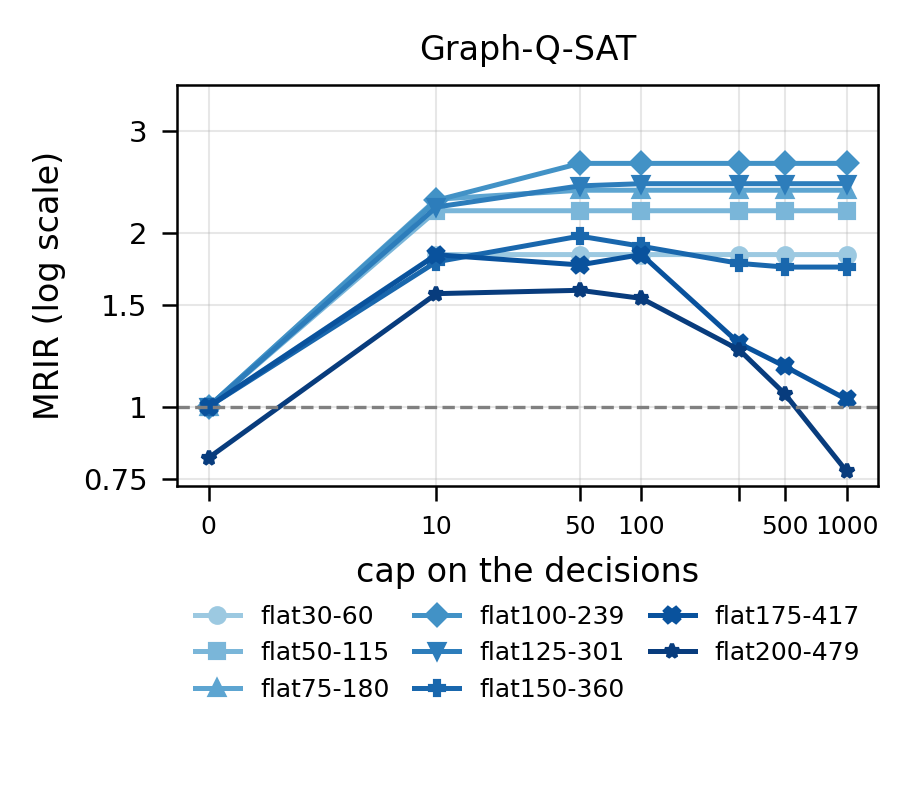
\includegraphics[width=\textwidth, height=\goldenpower{-1}\textheight,
        keepaspectratio]{graphqsat.png}
    \end{column}
    \begin{column}{0.5\textwidth}\centering
      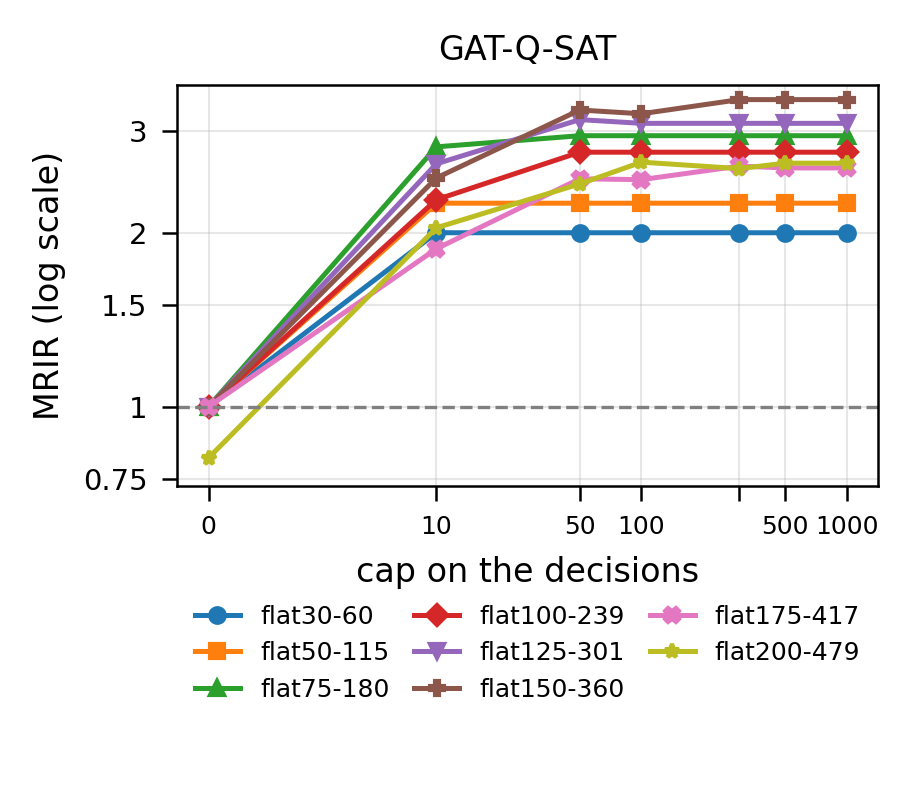
\includegraphics[width=\textwidth, height=\goldenpower{-1}\textheight,
        keepaspectratio]{gatqsat.png}
    \end{column}
  \end{columns}
  \vspace{1mm}
  {\footnotesize \T{Runs of 2021, one line per family, each in its color (the same in every figure); the point at cap 0
  is MiniSat without restarts. On the large families the decisions of Graph-Q-SAT after the
  first few tens make the search longer.}{Run del 2021, una linea per famiglia, ognuna nel suo colore (lo stesso in ogni figura); il punto al cap 0 \`e MiniSat senza restart. Sulle famiglie grandi le decisioni di
  Graph-Q-SAT dopo le prime decine allungano la ricerca.}\par}
\end{frame}

\begin{frame}{\T{Capacity or attention}{Capacit\`a o attenzione}}
  \upd{\T{[The four variants on the eight families, from Table 2 of the note: whether
  Graph-Q-SAT wide closes the gap, whether attention aggregation reaches GAT-Q-SAT at a sixth
  of its added parameters, and the size of the differences against the variation across
  the seeds.]}{[Le quattro varianti sulle otto famiglie, dalla tabella 2 della nota: se
  Graph-Q-SAT wide chiude il divario, se attention aggregation arriva a GAT-Q-SAT con un
  sesto dei suoi parametri aggiunti, e l'ampiezza delle differenze rispetto alla variazione
  fra i semi.]}}
\end{frame}

\begin{frame}{\T{Trained on random formulas, tested on graph coloring}{Addestrati su formule random, provati sul graph coloring}}
  \centering
  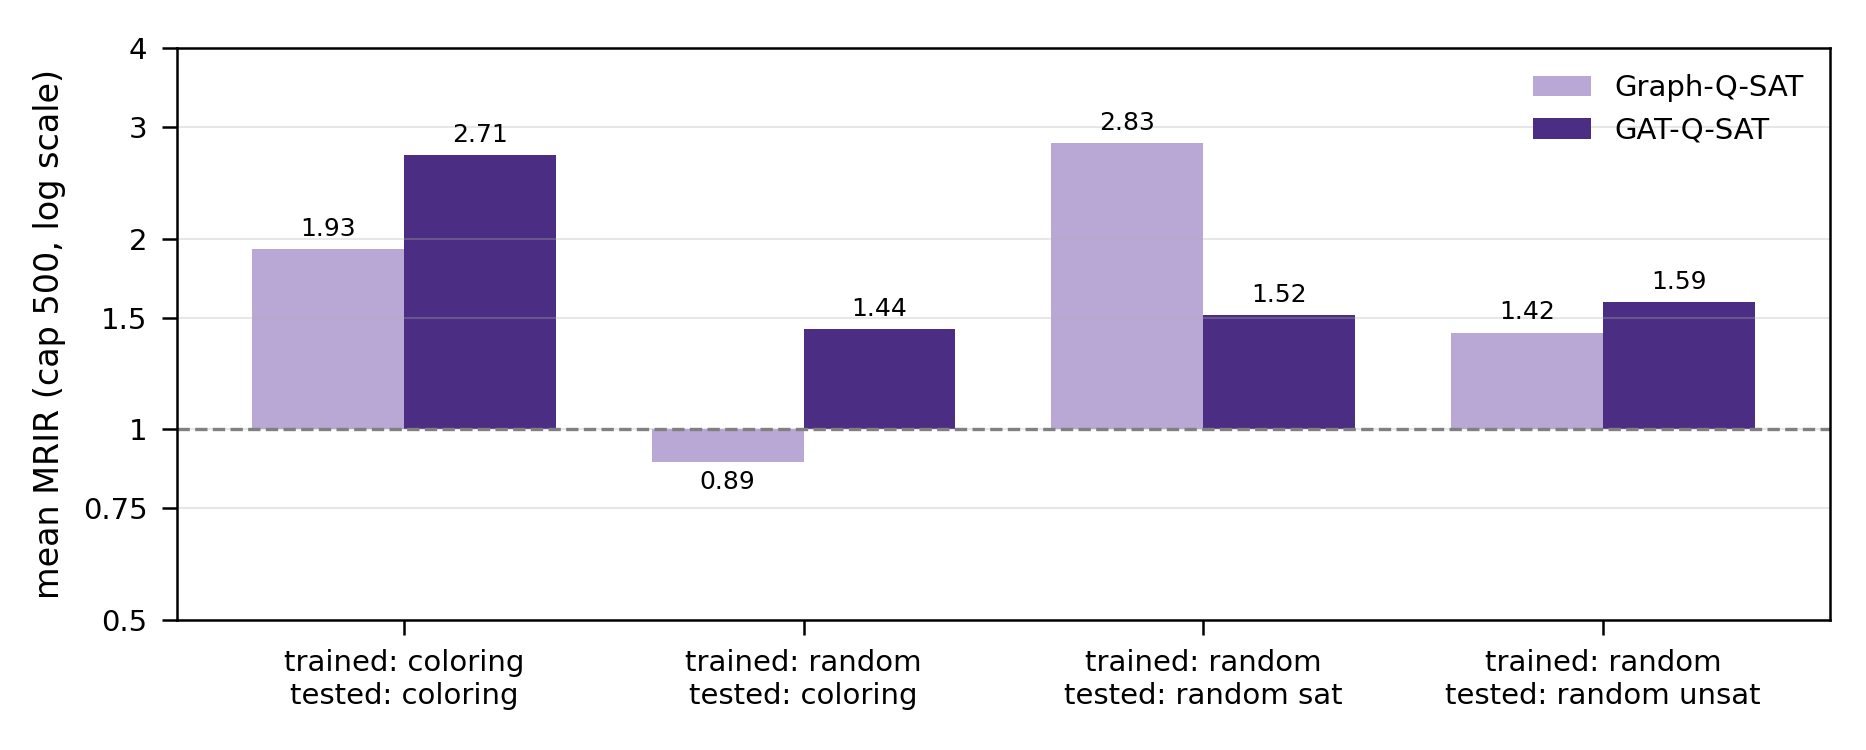
\includegraphics[width=0.92\textwidth, height=\goldenpower{-1}\textheight,
    keepaspectratio]{thesis.png}\\[1mm]
  \begin{columns}
    \begin{column}{0.92\textwidth}\footnotesize
      \T{Light gray Graph-Q-SAT, dark gray GAT-Q-SAT.
      Trained on uniform random 3-SAT, Graph-Q-SAT is below MiniSat on five of the eight
      coloring families, GAT-Q-SAT above it on seven: the weighting of the neighbors helps
      also on a structure not seen in training.}%
      {Grigio chiaro Graph-Q-SAT, grigio scuro GAT-Q-SAT.
      Addestrato sul random 3-SAT uniforme, Graph-Q-SAT \`e sotto MiniSat su cinque delle otto
      famiglie di coloring, GAT-Q-SAT sopra su sette: pesare i vicini aiuta anche su una
      struttura non vista in training.}
    \end{column}
  \end{columns}
\end{frame}

\begin{frame}{\T{A change of domain: thirteen SATLIB families}{Un cambio di dominio: tredici famiglie di SATLIB}}
  \begin{columns}[c]
    \begin{column}{0.6\textwidth}\centering
      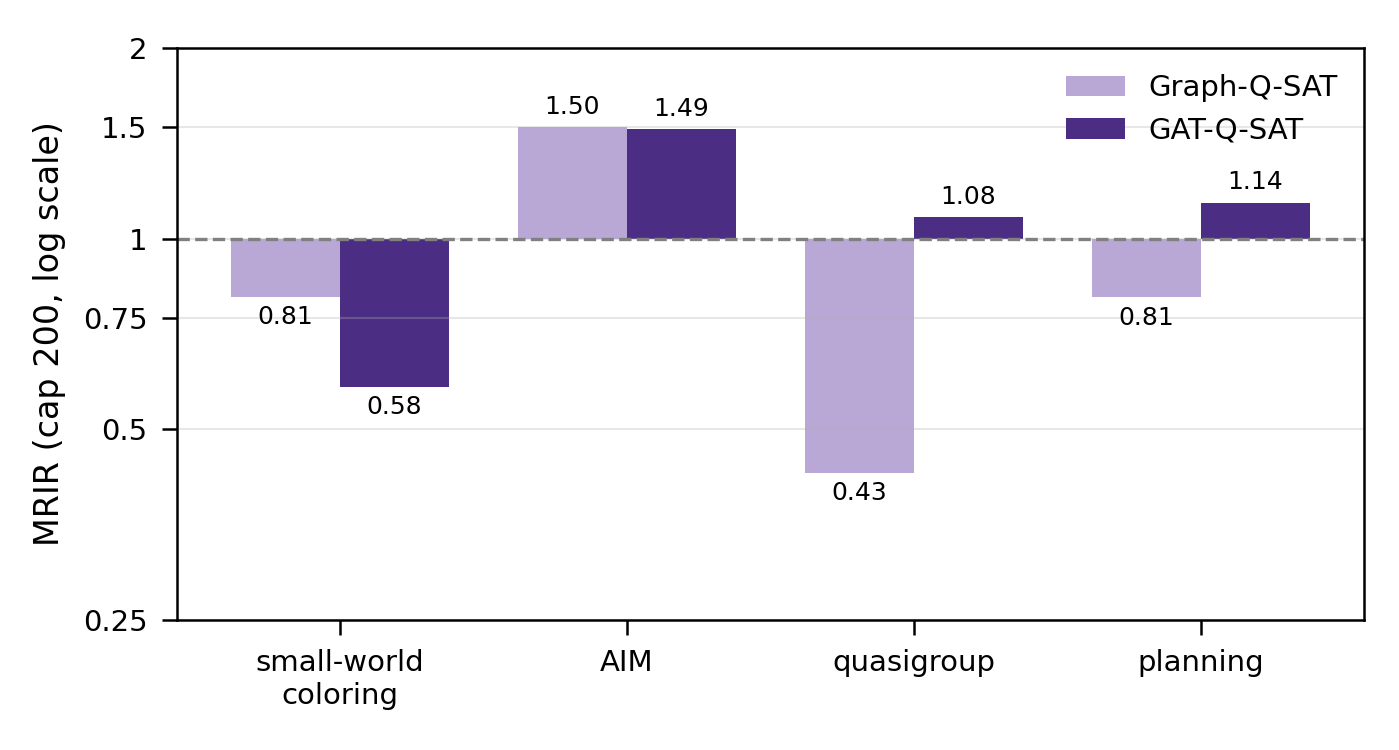
\includegraphics[width=\textwidth]{transfer.png}
    \end{column}
    \begin{column}{0.4\textwidth}\footnotesize
      \T{The coloring-trained models, with no retraining, on all the structured SATLIB
      families up to 2000 variables and 150000 clauses, and on small-world coloring at nine
      levels of rewiring; cap 200, MRIR against the stronger MiniSat.}%
      {I modelli addestrati sul coloring, senza riaddestramento, su tutte le famiglie
      strutturate di SATLIB fino a 2000 variabili e 150000 clausole, e sul coloring
      small-world a nove livelli di rewiring; cap 200, MRIR contro il MiniSat pi\`u forte.}\\[2mm]
      \upd{\T{[On how many families each variant is above MiniSat and above the others, and
      where the ranking flips.]}{[Su quante famiglie ogni variante \`e sopra MiniSat e sopra
      le altre, e dove l'ordine si inverte.]}}
    \end{column}
  \end{columns}
\end{frame}

\begin{frame}{\T{Uniform random 3-SAT: the ranking is reversed}{Random 3-SAT uniforme: l'ordine si inverte}}
  \begin{columns}
    \begin{column}{0.5\textwidth}\centering
      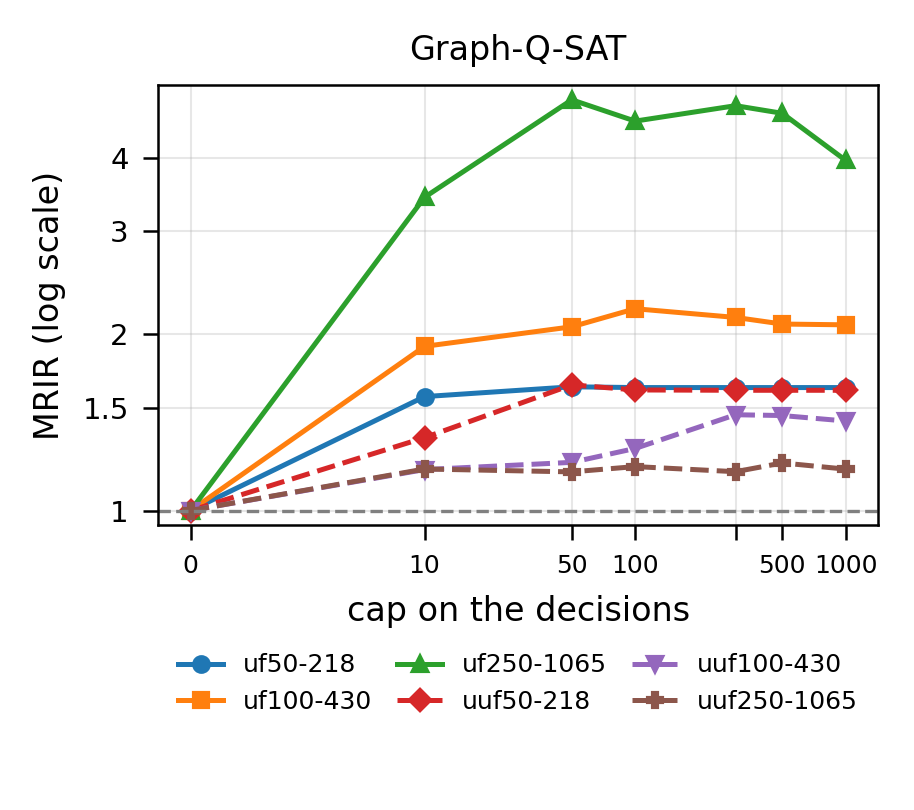
\includegraphics[width=\textwidth, height=\goldenpower{-1}\textheight,
        keepaspectratio]{graphqsat_random.png}
    \end{column}
    \begin{column}{0.5\textwidth}\centering
      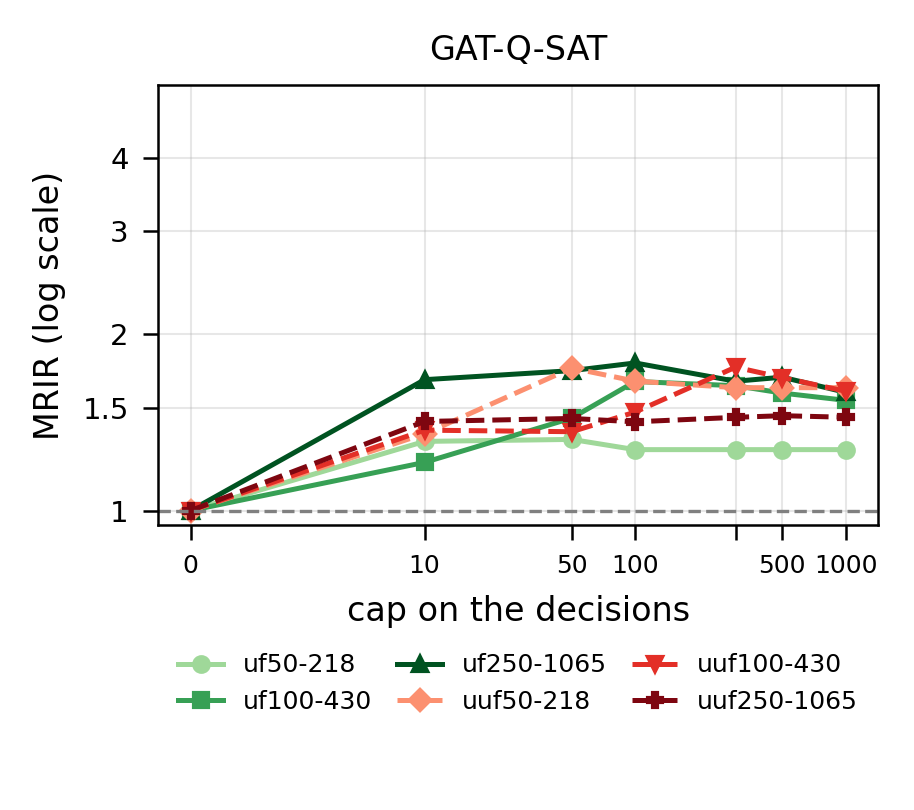
\includegraphics[width=\textwidth, height=\goldenpower{-1}\textheight,
        keepaspectratio]{gatqsat_random.png}
    \end{column}
  \end{columns}
  \vspace{1mm}
  {\footnotesize \T{On satisfiable formulas Graph-Q-SAT is better at all sizes ($4.78$ against
  $1.69$ at 250 variables): at the phase transition the neighbors of a node are statistically
  alike. On unsatisfiable formulas the two are level or GAT-Q-SAT is ahead.}{Sulle formule
  soddisfacibili Graph-Q-SAT \`e migliore a tutte le dimensioni ($4.78$ contro $1.69$ a 250
  variabili): alla transizione di fase i vicini di un nodo sono statisticamente uguali. Sulle
  insoddisfacibili i due sono alla pari o GAT-Q-SAT \`e avanti.}\par}
\end{frame}

\begin{frame}{\T{Iterations and running time}{Iterazioni e tempo}}
  \begin{center}\small
  \begin{tabular}{lcc@{\qquad}cc@{\qquad}cc}
    \toprule
     & \multicolumn{2}{c}{cap $50$} & \multicolumn{2}{c}{cap $500$} & \multicolumn{2}{c}{cap $1000$} \\
     & \T{sec}{sec} & MRIR & \T{sec}{sec} & MRIR & \T{sec}{sec} & MRIR \\
    \midrule
    Graph-Q-SAT & \upd{2.55} & \upd{1.59} & \upd{26.51} & \upd{1.05} & \upd{57.67} & \upd{0.77} \\
    GAT-Q-SAT   & \upd{3.52} & \upd{2.43} & \upd{12.20} & \upd{2.64} & \upd{12.19} & \upd{2.64} \\
    \bottomrule
  \end{tabular}\\[1mm]
  {\scriptsize \T{\texttt{flat200-479}, median seconds per instance}{\texttt{flat200-479}, secondi
  per istanza, mediana}}
  \end{center}
  \begin{itemize}
    \item \T{A decision of GAT-Q-SAT costs more, but at larger caps it is the faster of the
          two, since it terminates in fewer decisions.}%
          {Una decisione di GAT-Q-SAT costa di pi\`u, ma ai cap pi\`u alti \`e il pi\`u veloce
          dei due, perch\'e termina con meno decisioni.}
    \item \T{Both take seconds where MiniSat takes a fraction of a second: at this size
          neither is competitive in time, which is the motivation of the restricted
          heuristics (implemented, not measured) and of offline inference.}%
          {Entrambi impiegano secondi dove MiniSat impiega una frazione di secondo: a questa
          dimensione nessuno dei due \`e competitivo nel tempo, ed \`e la ragione delle
          euristiche ristrette (implementate, non misurate) e dell'inferenza offline.}
  \end{itemize}
\end{frame}

% ==================================================================== conclusions
\begin{frame}{\T{Conclusions and limits}{Conclusioni e limiti}}
  \begin{itemize}
    \item \T{On graph coloring GAT-Q-SAT took fewer decisions on every family, with a gap
          that grows with the size; it was also the better of the two when trained on random
          formulas and tested on coloring.}%
          {Sul graph coloring GAT-Q-SAT ha preso meno decisioni su ogni famiglia, con un
          divario che cresce con la dimensione; \`e stato il migliore dei due anche addestrato
          su formule random e provato sul coloring.}
    \item \upd{\T{[The controls: attention or capacity.]}{[I controlli: attenzione o capacit\`a.]}}
    \item \T{On satisfiable uniform random 3-SAT Graph-Q-SAT was clearly superior, where there
          is no structure for the attention to weight.}%
          {Sul random 3-SAT uniforme soddisfacibile Graph-Q-SAT \`e stato nettamente superiore,
          dove non c'\`e struttura che l'attenzione possa pesare.}
    \item \T{Limits: three seeds per model (two per control) do not resolve differences of a
          few tenths; neither model is competitive with MiniSat in time; the largest SATLIB
          instances (e.g., bounded model checking) are beyond the size I could evaluate.}%
          {Limiti: tre semi per modello (due per controllo) non bastano per differenze di pochi
          decimi; nessuno dei due modelli \`e competitivo con MiniSat nel tempo; le istanze pi\`u
          grandi di SATLIB (per esempio il bounded model checking) sono oltre la dimensione che
          ho potuto valutare.}
  \end{itemize}
  \vfill
  {\scriptsize \T{Code, instances and logs:}{Codice, istanze e log:}
  \href{https://github.com/dmeoli/GQSAT}{\texttt{github.com/dmeoli/GQSAT}}.}
\end{frame}

\begin{frame}[standout]
  \T{Thank you for your \emph{attention}!}{Grazie per l'\emph{attenzione}!}
  \par\vspace{\fib{8}pt}
  {\modularsize{-0.5}\mdseries
   \href{https://github.com/dmeoli/GQSAT}{\textcolor{lamalunga-on-primary}{\texttt{github.com/dmeoli/GQSAT}}}}
\end{frame}

\end{document}
